\documentclass[12pt]{article}
%Required: You must have these
\usepackage{graphicx}
\usepackage{tabularx}
\usepackage{natbib}
\usepackage{lineno}
\linenumbers

\usepackage{array}
\usepackage{amsmath}
%\usepackage[backend=bibtex]{biblatex}
\setkeys{Gin}{width=0.8\textwidth}
%\setlength{\captionmargin}{30pt}
\setlength{\abovecaptionskip}{10pt}
\setlength{\belowcaptionskip}{10pt}
 \topmargin -1.5cm 
 \oddsidemargin -0.04cm 
 \evensidemargin -0.04cm 
 \textwidth 16.59cm
 \textheight 21.94cm 
 \parskip 7.2pt 
\renewcommand{\baselinestretch}{1.2} 	
\parindent 0pt

\bibliographystyle{..//..//refs/bibstyles/amnat.bst}
\usepackage{xr-hyper}
\usepackage{hyperref}


\title{
Patterns of spring-freeze risk for temperature trees contributes to phenological cue differences, but leaves much unexplained\\
Other
}

\author{Dan, Cat, Nacho, Ben Cook, Faith, Deidre, Mira Geoff and Lizzie}
\usepackage{Sweave}
\begin{document}
\Sconcordance{concordance:rangeredo.tex:rangeredo.Rnw:%
1 35 1 1 0 103 1}

\maketitle

\section*{Abstract}
\section*{Introduction}

Phenology, the timing of annual life cycle events, allows for organisms to match critical life-cycle transitions with optimum environmental conditions. Through the phenology of spring budburst, temperate woody plants balance the resource and competition advantages of precocious leafout with the risk of damage from late season freezes \citep{Savage:2013aa}. To navigate this trade-off, woody plants have evolved complex physiological responses to sense environmental cues that signal the arrival of appropriate conditions for resuming growth \citep{Polgar2011}.Decades of research on phenology  suggest that warming spring temperatures (forcing), cool winter temperatures (chilling) and day length (photoperiod) are the primary environmental cues for woody plant phenology in temperate regions \citep{Ettinger:2020aa,Forrest2010}. These studies also demonstrate the there are substantial cue-use differences among species, with some species relying more heavily on some cues over others \citep{Laube:2014aa,Pau2011}. Yet, our knowledge about why species differ in their cue responses is currently limited, and better understanding the ecological and evolutionary drivers that shape phenological cues is critical for our ability to predict the magnitude and impacts of phenological shifts with climate change.


The predictability of the arrival spring may strongly influence the evolution of phenological cues \citep{Zohner:2017aa,Zohner:2017ua,Dawson2025}. In regions where the start of spring is unpredictable, species should evolve stronger dependence on chilling and photoperiod cues to prevent premature leafout and exposure to frost damage. In contrast, in regions where the seasonal warming reliably indicates the start of spring, species should respond strongly to forcing and not chilling or photoperiod. This spring predictability hypothesis (hereafter:SPH) is intuitive and has found some recent support in the literature \citep{Zohner:2017aa}. However, the SPH hinges on the assumption that species phenological responses are at a stable equilibrium with their environment, as assertion that is not well supported \citep{Normand2011,Lechowicz1984}. It is also unclear the time scale at which season predictability would shape cue responses. Spring predictability could drive selective pressure to increase chilling and/or photoperiod sensitivity on an evolutionary time scale, or define species ranges based on their inherited cue sensitivities on an ecological time scale. Testing the predictions of SPH across multiple geographic scales can serve to evaluate this hypothesis, and offer an improved understanding of the drivers of biogeographic patterns of phenology cue sensitivity.

\section*{Continental Climatic Pattern}

Global circulation patterns generate substantially different spring climatic conditions on either side of the North Atlantic \citep{}. In Eastern North America, the spring is marked by instability, while in Europe, the arrival of spring is generally more consistent (Figure \ref{fig:mappy}). Given these contrasting climate regimes, the SPH predicts that North American species should have stronger sensitivity to chilling and photoperiod and weaker to forcing \citep{Dawson2025}. We tested these predictions using phenological observations from the Observed Spring Phenology Responses in Experimental Environments  (OSPREE database \citep{wolkovich2019}) with Bayesian Hierarchical models developed by \citet{Morales-Castilla:2024vp} to estimate species level cues and account for phylogeny. We compared the cue sensitivities of North American and Europe species by extracted all species-level posterior samples for forcing, chilling and photoperiod sensitivity and grouping them by the continent to which species' were native (See Supporting Information: Methods for details).

There were no substantial differences in cue sensitivity between continents (Figure: \ref{fig:cont}). Mean forcing sensitivity for European species was -6.76 UI_{95}(-17.80,2.08)  and -7.94 UI_{95}(-17.90,1.93) for North American species. Mean chilling sensitivity for European species was -8.44 UI_{95}(-22.60,4.69) and -8.76 UI_{95}(-26.90,4.82) for North American species. Mean photoperiod sensitivity for European species was -1.36 UI_{95}(-5.91,2.89) and -1.35 UI_{95}(-5.88,2.98) for North American species.

This finding does not support to the SPH, though it is not particularly surprising given that recent studies have found there to be strong phylogenetic conservatism in phenological cue responses, and that there are many closely related congeners found in both North America and Europe. It is therefore likely that patterns of cue use diverged among taxa well before the modern placement of continents, under different climate conditions than North America and Europe experience today. (wow say better). These results call into question the recent assertion that European plant species successfully invade North American ecosystems because their higher reliance on forcing cues allows them to leafout earlier and gain a growth advantage over their competitors \citep{Dawson2025}. While these kinds phenological priority effects have been documented as contributing to the success of invaders \citep{Buonaiuto:2023wy,Alexander2019} our findings indicate that other mechanisms are likely more important for explaining the success of European woody plants in North America. Instead, this finding may help us understand why many European timber species have been successfully established in Northern America (and visa versa), without becoming aggressive on the landscape. We should note that when we subset this analysis to include only the 29 for which we could find well developed range maps, we did in-fact observe European species to have a weaker chilling sensitivity (Figure S1, need to make it), which may further explain the pervasiveness of the idea that European invaders are successful in North America due to weaker secondary phenological cues.

\section*{Range Patterns}
Instead of continental-scale patterns of biogeography driving divergent evolutionary trajectories of cue use, it is also possible that phenological responses to cues play a more important role in determining species range limits \citep{Chuine2010}. The distributions of species that rely primarily on forcing, should be restricted geographic regions where spring predictability is high, while species that rely more heavily on chilling and photoperiod can persist in regions where spring predictability is low. If this is the case, the SPH predicts that within each continent, species with higher chilling and photoperiod cue responses should be associated with lower spring predictability across their ranges.

We tested this prediction by regressing the species-level posterior estimates of forcing, chilling and photoperiod sensitivity from our previously described model against the two metrics of spring predictability: Spring Temperature Variability (STV), defined as the standard deviation of mean minimum temperature from March-May \citep[See Supporting Information Methods][]{Zohner:2017aa}, and the standard deviation in growing degree days to last frost. We analyzed this relationship between spring predictability and cue responses using a Bayesian hierarchical framework, with separate models for each cue by continent (see Supporting Information: Methods for details). 

With STV as the metric for spring predictability, we found that in Europe---spring predictability across a species' range had no clear relationship to forcing or photoperiod cues cues (mean forcing effect: -0.59, UI_{95}[-4.44,3,01], mean photoperiod effect: 1.34, UI_{95}[-0.49, 3.24]). Contrary to the predictor of the SPH, decreasing spring predictability was associated with weaker chilling sensitivity (mean chilling effect: 6.37, UI_{95}[3.99, 7.97]). For North American species, spring predictability also had no clear relationship to forcing or photoperiod cue sensitivity (mean forcing effect: -0.05, UI{95}[-2.26, 2.06], mean photoperiod effect: 0.15 UI_{95}[-0.93, 1.21]). For chilling, decreasing spring predictability was associated with increased chilling sensitivity (mean chilling effect: -3.45, UI_{95}[-7.50, 0.69]), supporting the prediction of the SPH.

These patterns qualitatively match the previous findings from \citet{Zohner:2017aa}, that report stronger reliance on secondary cues (i.e. chilling) in North American compared to Europe based on the substantial differences in STV between the continents. While STV may be a reasonable proxy for spring predictability in many cases, it does not capture the within-season variability in frost risk that is what actually drives environmental filtering on phenological cues. A measure of variability in the number of growing degree days before the last frost is a more biologically realistic proxy for spring predictability (HELP HERE).

With standard deviation in growing degree days to last frost as the metric for spring predictability, we observed different relationships between spring predictability and species-level cue sensitivity than we found using STV. For European species, we found decreasing spring predictability was associated with both higher forcing sensitivity (mean forcing effect: -3.61, UI_{95}[9.04, 1.64]) and chilling sensitivity (mean chilling effect: -5.27, UI_{95}[11.45, 1.36]), while there was no clear effect of spring predictability on photoperiod sensitivity (mean photoperiod sensitivity:-0.80, UI_{95}[-3.62, 2.09]). In interpreting these relationships, it is important to recognize that the amount of variation in GDDs to last frost in Europe is very small (0.62 to 2.97), especially when compared to North America (13.68 to 56.01). This suggest that the arrival of spring in Europe is always relatively predictably from a growing degree day perspective, and we should exhibit caution in putting too much biological stock in the statistical association between European spring predictability and chilling cue sensitivity.

For North American species, decreased predictability was associated with weaker forcing sensitive though the strength of this association was relatively weak (mean forcing effect: 0.09 UI_{95}[-0.04,0.24]). There was no clear relationship between spring predictability and chilling sensitivity (mean chilling effect: -0.02 UI_{95}[-0.34, 0.31]). For photoperiod sensitivity, we observed a moderate association between decreasing spring predictability and photoperiod sensitivity (mean photoperiod effect: -0.04, UI_{95}[-0.11, 0.04]). This observed relationship between spring predictability and photoperiod match the expectations of the SPH. Photoperiod is generally the weakest cue influencing spring phenology \citep{Ettinger:2020aa}, and there is comparatively little inter-specific variation in cue strength compared to forcing and chilling \citep{Morales-Castilla:2024vp}. 

In sum, our analyses of the relationships between spring predictability and phenological sensitivity to forcing, chilling and photoperiod offer only marginal support for the SPH. For North American species, less spring predictability was associated with an increased reliance on chilling (i.e. chilling sensitivity) when we used STV as a metric of predictability and and increased reliance on photoperiod when we used Stdv in GDDs to last frost as a metric of spring predictability. For European species spring predictability was associated with increased reliance on chilling (i.e. stronger chilling sensitivity) when we used Stdv in GDDs to last frost as a metric of predictability, though as we caution above, we feel that given the low levels of variability in in GDDs to last frost observed in Europe, it is difficult to claim such low levels of variation would exert strong filtering pressure on species' ranges. While these three facets of the predictability/cue relationship support the expectations of the SPH, all other aspects of the predictability/cue relationship either show no relationship (i.e. forcing \& photoperiod effects with STV in Europe \& North America) or observed relationships contrary to the expectations of the SPH (i.e., chilling in Europe with STV and forcing in North America with Stdv. GDDs). We argue that these mixed results should not serve to refute the claims of the SPH---it is clear that spring predictability has a role to play in shaping where and how species successfully leaf out. However, our study indicates a more complicated picture of the factors that shape species' level differences in phenological cues. We discuss these aspects in the sections below.


\section*{Does local adaptation swamp the SPH?}
One possible reason for the weak support for the SPH we found in our analyses is that local adaptation in phenological cue sensitivity overwhelms any relationship between species-level cue use and range-wide climate conditions. There is currently a debate about the extent to which local adaptation shapes phenological cues \citep{Zeng2024}, and it is likely the strength of local adaptation varies among species, and phenological phases themselves \citep{Zeng2024,Savolainen2007}. However, if cues are locally adapted, it follows that neither continental differences or range wide climate conditions would be strongly associated with cue use. 

To assess this possibility in our data, we designed a two-level, hierarchical model for studies in the OSPREE database that sampled species from multiple provenance locations. We model study, species and population as intercepts, forcing and photoperiod as predictors (fixed effects) with species nested within population (i.e., site) as modeled groups (random effects). While we detected limited population level variation in forcing and photoperiod cue sensitivity, though this within species variation was less substantial than among species variation (Fig. \ref{fig:popy}). Notably, we found the largest source of variation in phenological cue estimates was the study effect Fig. \ref{fig:popy}). This result does not support the assertion that local adaptation is masking relationships between cue sensitivity and range-level climatic patterns.

\section*{Phenological cue differences: More than climate drivers}

Our study indicates that predictability of spring species' experience across their geographic ranges may play a role in shaping phenological cue sensitivities, there must be more to the story. When considering the fact that many species with divergent phenological cue sensitives have highly overlapping ranges (Make Figure S2) and experience similar environmental conditions (i.e., spring predictability, late season frost risk, etc) across their ranges, it is worthwhile to consider phenological cues in a community context \citep{}.

\textbf{I am hoping Deirdre and Lizzie have capacity to write a paragraph or two here basically phenology should be considered like a functional trait in that they not only relate to resource aquistion/growth/ surivvial but also do niche stuff and therefore end up under stabalizing selection though competition and species interactions}



\section{Conclusion:}
In this study we found limited support for the assertion that the predictability of spring shaping their relative reliance on forcing, chilling and photoperiod cues for spring phenology. Our results suggest that climate variability may drive cue use pattern only when it is sufficiently high, like in contemporary North America. These results suggests that future studies of phenological cue-use would benefit from a holistic integration of these bio-climatic hypotheses with phylogenetic, functional trait, and climatic legacy hypotheses to fully understand the evolution of phenological cues in woody plants, and how cue use patterns will impact species performance in the face of global change at across multiple spatial and temporal scales.

\bibliography{..//..//refs/ranges.bib}
\section*{Figures}

\begin{figure}[h!]
    \centering
 \includegraphics[width=\textwidth]{..//..//analyses/ranges/figures/concept figure maps with SDev of GDDlf.png} 
    \caption{Contrasting patterns of spring predictability in North America and Europe.}
    \label{fig:mappy}
\end{figure}


\begin{figure}[h!]
    \centering
 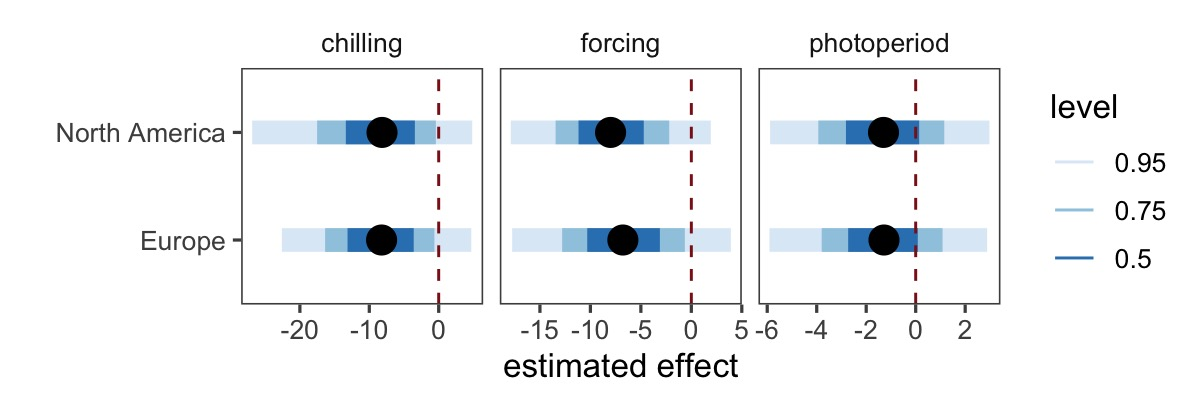
\includegraphics[width=\textwidth]{..//..//analyses/ranges/figures/NAvEuPMM.jpeg} 
    \caption{No difference between continents}
    \label{fig:cont}
\end{figure}

\begin{figure}[h!]
    \centering
 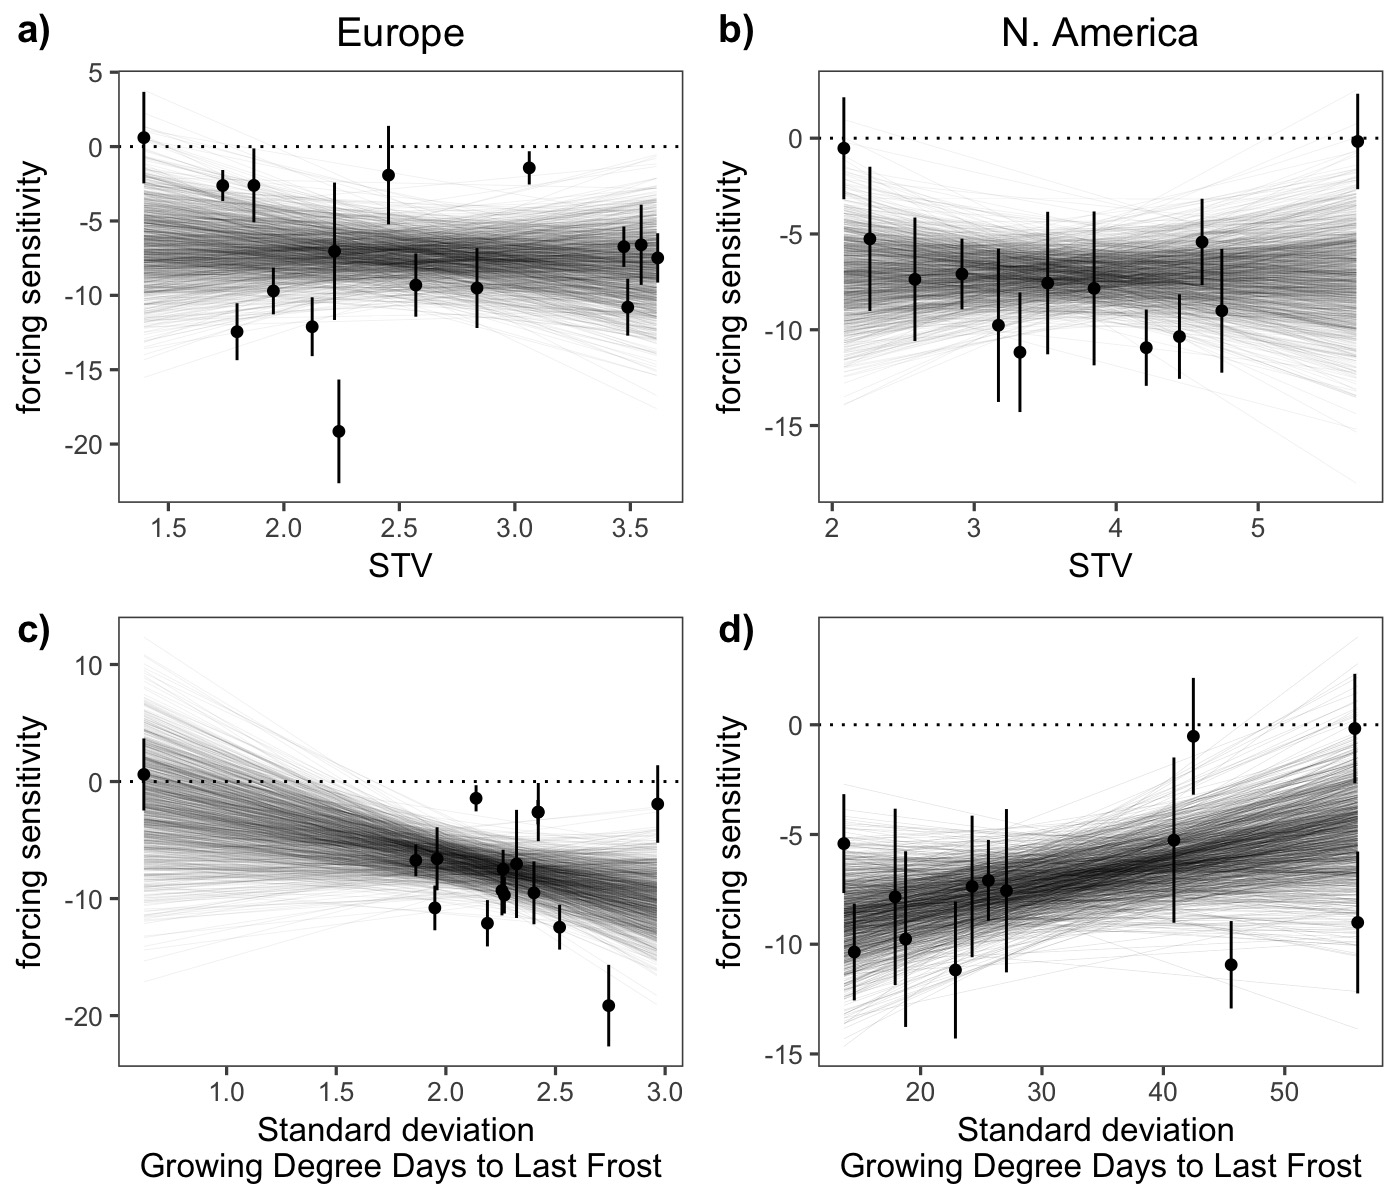
\includegraphics[width=\textwidth]{..//..//analyses/ranges/figures/contz_force.jpeg} 
    \caption{Forcing}
    \label{fig:force}
\end{figure}

\begin{figure}[h!]
    \centering
 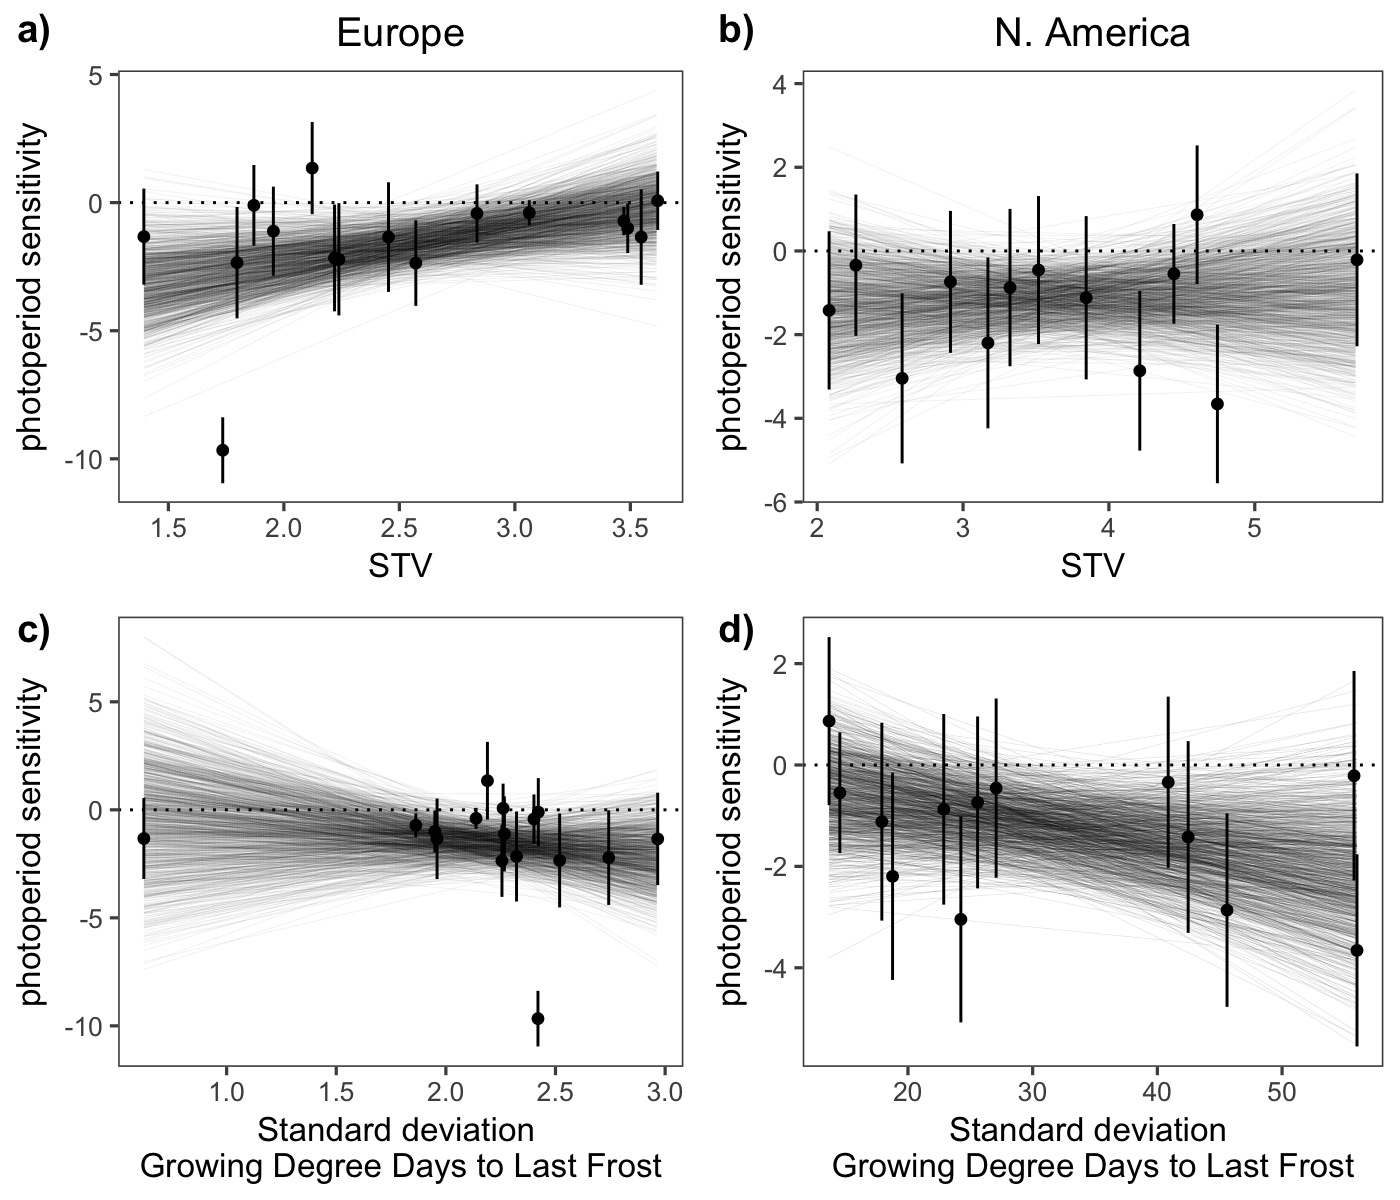
\includegraphics[width=\textwidth]{..//..//analyses/ranges/figures/contz_photo.jpeg} 
    \caption{Photoperiod}
    \label{fig:photo}
\end{figure}

\begin{figure}[h!]
    \centering
 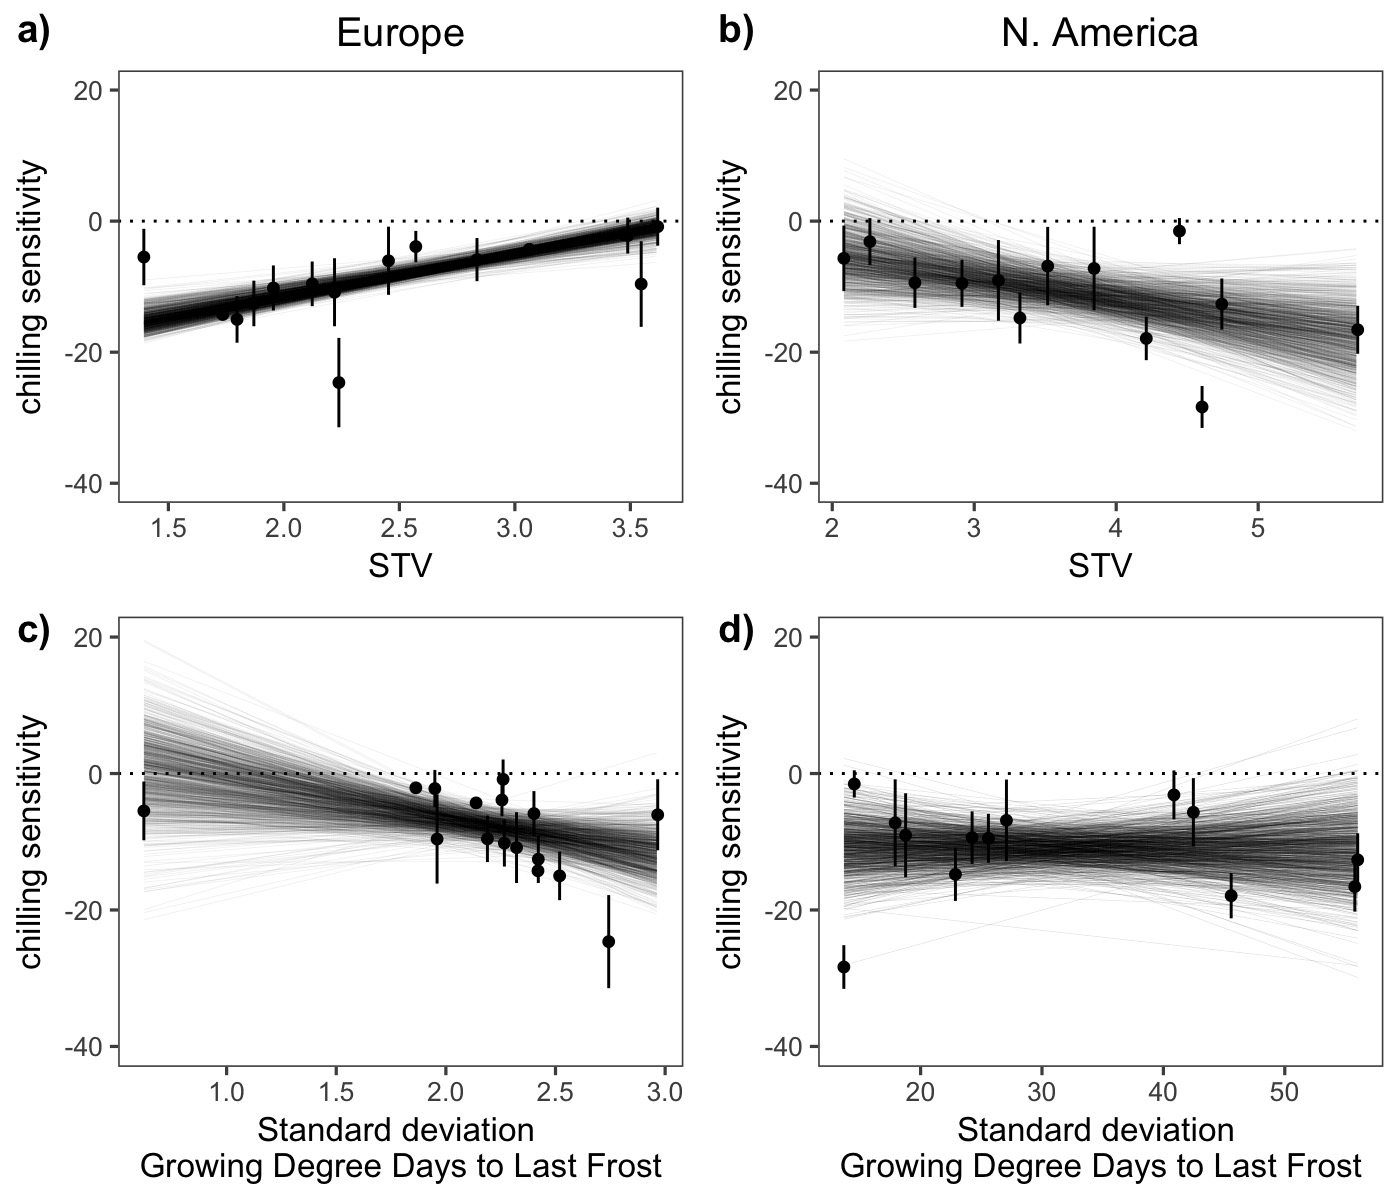
\includegraphics[width=\textwidth]{..//..//analyses/ranges/figures/contz_chill.jpeg} 
    \caption{Chilling}
    \label{fig:chill}
\end{figure}


\begin{figure}[h!]
    \centering
 \includegraphics[width=\textwidth]{..//..//analyses/ranges/figures/variancepartitioning.pdf} 
    \caption{ \textbf{Local adaptation model estimates of variation partitioning in the intercept and forcing and photoperiod predictors using the OSPREE dataset}. For both the forcing and photoperiod predictors, within species (intra-specific) variation is much smaller than across species (inter-specific) variation. Here we see that inter-specific variation exceeds intra-specific variation at the intercept-level as well but variation at the study level is largest, suggesting experimental design is driving the highest level of uncertainty.}
    \label{fig:popy}
\end{figure}

\end{document}
